\documentclass[10pt,nofootinbib]{revtex4}
\usepackage{amsmath,amssymb,amsfonts,mathrsfs,bm,dsfont}
\usepackage{enumerate}
\usepackage[all]{xy}
\usepackage[normalem]{ulem}	% delete line
\usepackage{graphics,color}
\usepackage{tikz}
	\usetikzlibrary{calc}
	\usetikzlibrary{decorations.markings}
	\usetikzlibrary{arrows}
	\usetikzlibrary{patterns}
\usepackage{pgfplots}


%\usepackage{hyperref}
\usepackage{feynmp} % feymann diagram
\usepackage{extarrows}


\newcommand*\dd{\mathop{}\!\mathrm{d}}
\newcounter{Claim}[section]
\newenvironment{Claim}[1][]{{\par\normalfont\bfseries \underline{Claim~\stepcounter{Claim}\arabic{Claim}.}~#1~~}}{\par}
\newcounter{Proposition}[section]
\newenvironment{Proposition}[1][]{{\par\normalfont\bfseries \underline{Proposition~\stepcounter{Proposition}\arabic{Proposition}.}~#1~~}}{\par}
\newcounter{Note}[section]
\newenvironment{Note}[1][]{{\par\normalfont\bfseries \underline{Note~\stepcounter{Note}\arabic{Note}.}~#1~~}}{\par}
\newcounter{Lemma}[section]
\newenvironment{Lemma}[1][]{{\par\normalfont\bfseries \underline{Lemma~\stepcounter{Lemma}\arabic{Lemma}.}~#1~~}}{\par}
\newcounter{Corollary}[section]
\newenvironment{Corollary}[1][]{{\par\normalfont\bfseries \underline{Corollary~\stepcounter{Corollary}\arabic{Corollary}.}~#1~~}}{\par}
\newenvironment{Proof}{{\par~{\normalfont\bfseries $\vartriangleright$}~~}}{\hfill $\square$\par\hfill\par} %\par
\newcounter{Def}[section]
\newenvironment{Def}[1][]{{\par\normalfont\bfseries \underline{Definition~\stepcounter{Def}\arabic{Def}.}~#1~~}}{\par}

\allowdisplaybreaks[4] %允许 align 跨页编排

\def\Re{\mathop{\mathcal{R}e}}
\def\Im{\mathop{\mathcal{I}m}}
\def\imp{\text{imp}}

\def\arrow{\tikz[scale=0.1,baseline=.1ex]{
	\draw[fill=black,rotate=-90] (-0.7,0)--(0,2)--(0.7,0);}
	}

\def\cross{\tikz[scale=0.1,baseline=.1ex]{
	\draw[thick,rotate=45] (-1,0)--(1,0);
	\draw[thick,rotate=45] (0,-1)--(0,1);}
	}





\begin{document}
\title{Conformal Field Theory and Applications in Condensed Matter Physics}% Force line breaks with \\
%\thanks{This is a reminiscent note for Hubbard-Stratonovich Transformation.}%

\author{Xiaodong Hu}
%\altaffiliation[Also at ]{Boson College}
\email{xiaodong.hu@bc.edu}
\affiliation{Department of Physics, Boston College}

\date{\today}

\begin{abstract}
	This is a research note about CFT. Particularly, we are interested the application beyond critical points around phase transitions.
\end{abstract}
\maketitle
\tableofcontents
\section{General Conformal Transformation}
	Let us consider a local field theory defined on a $D$-dimensional spacetime with \emph{Euclidean} metric $g_{\mu\mu}\equiv\eta_{\mu\nu}$ and signature $(p,q)$. A general diffeomorphism transform the metric to 
	\begin{equation*}
		g_{\mu\nu}\mapsto \widetilde{g}_{\mu\nu}(\widetilde{x} )\equiv\dfrac{\partial x_\mu }{\partial \widetilde{x}_\alpha }\dfrac{\partial x_\alpha}{\partial \widetilde{x}_\beta }g_{\alpha\beta}.
	\end{equation*}
	\begin{Def}[(Conformal Group)]
		Conformal transformation forms the subgroup of diffeomorphism group leaving the metric tensor unchcanged up to a scale factor
		\begin{equation}\label{1.1.1}
			\widetilde{g}_{\mu\nu}(\widetilde{x})=\Omega(x)g_{\mu\nu}(x). 
		\end{equation}
		Clearly Poincare group ($\Omega\equiv1$) is the subgroup of our confromal group.
	\end{Def}
	To find out all generators of conformal transformation, we should look at the infinitesimal transformation $\widetilde{x}_\mu\equiv x_\mu+\varepsilon_\mu+\mathcal{O}(\varepsilon^2) $ so that
	\begin{align*}
		\widetilde{g}_{\mu\nu} &\equiv(\delta^\alpha_\mu+\partial_\mu \varepsilon^\alpha)(\delta^\beta_\nu+\partial_\nu \varepsilon^\beta)g_{\alpha \beta}=g_{\mu\nu}+\partial_\mu \varepsilon^\alpha g_{\alpha\nu}+\partial_\nu \varepsilon^\beta g_{\mu \beta}+\mathcal{O}(\varepsilon^2)\\
		&=g_{\mu\nu}+(\partial_\mu \varepsilon_\nu+\partial_\nu \varepsilon_\mu)+\mathcal{O}(\varepsilon^2)
	\end{align*}
	Definition \eqref{1.1.1} demands
	\begin{equation}\label{1.1.2}
		(\partial_\mu \varepsilon_\nu+\partial_\nu \varepsilon_\mu)=(\Omega(x)-1)g_{\mu\nu}\equiv K(x)g_{\mu\nu},
	\end{equation}
	mutiplying $g^{\mu\nu}$ on the left we have
	\begin{equation*}
		2\partial^\mu \varepsilon_\mu=K(x)D.
	\end{equation*}
	In combination of \eqref{1.1.2} again we can cancel the undetermined scaling factor $\Omega(x)$ and obtain the constraint equation of conformal generators
	\begin{equation}\label{1.1.3}
		\boxed{(\partial_\mu \varepsilon_\nu+\partial_\nu \varepsilon_\mu)=\dfrac{2}{D}(\partial \cdot \varepsilon)g_{\mu\nu}.}
	\end{equation}
	\indent To reveal the particularity of dimensionality-dependence we need to re-arrange equation \eqref{1.1.3} to a more explicit form. Applying $\partial^\nu$ and $\partial_\nu$ on \eqref{1.1.3} gives
	\begin{equation}\label{1.1.4}
		\partial_\mu\partial_\nu(\partial \cdot \varepsilon)+\partial^2\partial_\nu\varepsilon_\mu=\dfrac{2}{D}\partial_\mu \partial_\nu(\partial\cdot\varepsilon).
	\end{equation}
	Similarly for twice derivatives of $\partial_\mu$ and $\partial^\mu$ we have
	\begin{equation}\label{1.1.5}
		\partial^2\partial_\mu\varepsilon_\nu+\partial_\nu\partial_\mu(\partial \cdot \varepsilon)=\dfrac{2}{D}\partial_\nu \partial_\mu(\partial\cdot\varepsilon).
	\end{equation}
	Adding \eqref{1.1.4} and \eqref{1.1.5} up and utilize \eqref{1.1.3} we get the differential equation of $(\partial\cdot\varepsilon)$
	\begin{equation}\label{1.1.6}
		2\partial_\mu \partial_\nu(\partial\cdot\varepsilon)+\partial^2\left(\dfrac{2}{D}(\partial\cdot \varepsilon)g_{\mu\nu}\right)=\dfrac{4}{D}\partial_\mu \partial_\nu(\partial\cdot\varepsilon)\implies (g_{\mu\nu}\partial^2+(D-2)\partial_\mu \partial_\nu)(\partial\cdot \varepsilon)=0,
	\end{equation}
	or ({\color{red}if $D\neq2$})
	\begin{equation*}
		(D-1)\partial^2(\partial \cdot \varepsilon)=0
	\end{equation*}
	if we multiply $g^{\mu\nu}$ on the left hand side.\par
	Clearly if $D=1$ the above constraint equation degenerates and the theory is trivial. So we only focus on the case when $D\geq2$.

	\subsection{Conformal Transformation in $D>2$}
		For $D>2$ constraint \eqref{1.1.6} implies that $\varepsilon_\mu$ is at most \emph{quadratic} in coordinate
		\begin{equation*}
			\varepsilon_\mu=a_\mu+b_{\mu\nu}x^\nu+c_{\mu\nu\rho}x^\nu x^\rho
		\end{equation*}
		with $c_{\mu\nu\rho}\equiv c_{\mu\rho\nu}$.\par
		\begin{enumerate}[1)]
			\item Clearly $\varepsilon_\mu=a_\mu$ represents space-time \textbf{translation} $x'_\mu\mapsto x_\mu+a_\mu$ as ususal.
			\item By inserting $\varepsilon_\mu=b_{\mu\nu}x^\nu$ back into \eqref{1.1.3} we obtain
				\begin{equation*}
					b_{\mu\nu}+b_{\nu\mu}=\dfrac{2}{D}(b_{\alpha\beta} \partial^\alpha x^\beta)\eta_{\mu\nu}.
				\end{equation*}
				Separating $b_{\mu\nu}$ into symmetric part $b^s_{\mu\nu}\equiv b^s_{\mu\nu}$ and anti-symmetric part $b^a_{\mu\nu}\equiv-b^a_{\mu\nu}$, one can immediately finds out that $b^s_{\mu\nu}$ must be a pure trace
				\begin{align*}
					2b^s_{\mu\nu}=\dfrac{2}{D}(b^s)_{\alpha}^{~\alpha}\eta_{\mu\nu}\implies b^s_{\mu\nu}\propto\eta_{\mu\nu},
				\end{align*}
				which is called space-time \textbf{dilation}, while we have no constraint on space-time \textbf{rotation} $b^a_{\mu\nu}\equiv\omega_{\mu\nu}$.
			\item By inserting $\varepsilon_\mu=c_{\mu \alpha\beta}x^\alpha x^\beta$ back into \eqref{1.1.3} we have
				\begin{equation*}
					c_{\mu\nu\beta}x^\beta+c_{\nu\mu\beta}x^\beta=\dfrac{2}{D}c^\alpha_{~\alpha\beta}x^\beta g_{\mu\nu}.
				\end{equation*}
				To express $c_{\mu\nu\beta}$ explicitly, we have to cycle all the indices, summing and subtracting them with symmetric condition on the latter two indices of $c_{\mu\nu\beta}$, which yields the \textbf{special conformation transformation} (SCT)
				\begin{equation*}
					c_{\mu\nu\beta}=\dfrac{1}{D}(c^\alpha_{~\alpha\beta}g_{\mu\nu}+c^\alpha_{~\alpha\nu}g_{\mu\beta}-c^\alpha_{~\alpha\mu}g_{\nu\beta})\equiv b_\beta\eta_{\mu\nu}+b_\nu\eta_{\mu\beta}-b_\mu\eta_{\nu\beta},
				\end{equation*}
				where $b_\beta\equiv c^\alpha_{~\alpha\beta}/D$.
		\end{enumerate}
		In summary, we get four kinds of finite conformal transformation as table \ref{tab:1}. And the corresponding four kinds of infinitesimal transformation is also shown in table \ref{tab:2} by taking the \emph{tagent mapping}\footnote{Generally the generator for infinitesimal transformation keeping field configuration unchanged $\Phi'(x')=\Phi(x)$ and parameterized by $\omega_a$ is given by \begin{equation*}
			iG_a\equiv\dfrac{\delta x^\mu}{\delta \omega_a}\partial_\mu.
		\end{equation*}} of $x'_\mu(x)$.
		\begin{table}
			\begin{tabular}{p{3cm}p{12cm}}
				%\hline
				Translation&$x'_\mu= x_\mu+a_\mu$\\[0.6em]
				Dilation&$x'_\mu= x_\mu+\dfrac{2}{D}(b^s)^\alpha_{~\alpha}\eta_{\mu\nu}x^\nu\equiv(1+\alpha)x_\mu$\\[0.6em]
				Rotation&$x'_\mu= x_\mu+\omega_{\mu\nu}x^\nu$\\[0.6em]
				SCT&$x'_\mu= x_\mu+(b_\beta\eta_{\mu\nu}+b_\nu\eta_{\mu\beta}-b_\mu\eta_{\nu\beta})x^\nu x^\beta\equiv x_\mu+2(b\cdot x)x_\mu-b_\mu x^2$
				%\\[0.6em]
				%\hline
			\end{tabular}
			\caption{Four kinds of finite conformal transformations.}
			\label{tab:1}
		\end{table}
		\begin{table}
			\begin{tabular}{p{3cm}p{12cm}}
				Translation&$P^\alpha=-i\dfrac{\delta}{\delta a_\alpha}(x_\mu+a_\mu)\partial^\mu=-i \partial^\alpha$\\[0.6em]
				Dilation&$D=-i\dfrac{\delta}{\delta \alpha}(1+\alpha)x_\mu \partial^\mu=-ix^\mu \partial_\mu$\\[0.6em]
				Rotation&$L^{\alpha \beta}=-i\dfrac{\delta}{\delta \omega_{\alpha \beta}}(x_\mu+\omega_{\mu\nu}x^\nu) \partial^\mu=-i(\delta_{\alpha\mu}\delta_{\beta\nu}-\delta_{\alpha\nu}\delta_{\beta\mu})x^\nu \partial^\mu=i(x^\alpha \partial^\beta-x^\beta \partial^\alpha)$\\[0.6em]
				SCT&$K^\alpha=-i\dfrac{\delta}{\delta b_\alpha}(x_\mu+2(b\cdot x)x_\mu-b_\mu x^2)\partial^\mu=-i(2 x^\alpha (x\cdot \partial )-x^2 \partial^\alpha)$
			\end{tabular}
			\caption{Corresponding four generators of four kinds of conformal transformation.}
			\label{tab:2}
		\end{table}
	\subsection{Conformal Transformation in $D=2$}
		For $D=2$, constraint equation \eqref{1.1.3} reduces to simple
		\begin{equation}\label{1.2.1}
			\partial_1 \varepsilon_2\equiv-\partial_2 \varepsilon_1,\quad \partial_1 \varepsilon_1\equiv \partial_2 \varepsilon_2.
		\end{equation}
		which is nothing but celebrated \emph{Cauchy-Riemann equation} appearing in complex analysis. Particularly, if we introduce two conjugate complex variables $z\equiv x_1+ix_2$ and $\bar z\equiv x_1-i x_2$, constraint equation \eqref{1.2.1} tells us that two-dimensional conformal transformation decouple each other and are generated by nothing but \emph{holomorphic} and \emph{anti-holomorphic} functions $\varepsilon\equiv \varepsilon_1+i\varepsilon_2$ and $\bar \varepsilon=\varepsilon_1-i \varepsilon_2$ as following
		\begin{equation*}
			z\mapsto z'= z+\varepsilon(z),\quad \bar z\mapsto \bar z'=\bar z+\bar\varepsilon(\bar z),
		\end{equation*}
		where generally $\varepsilon(z)=\sum_n\alpha_n z^{n+1}$ and $\varepsilon(\bar z)=\sum_n\beta_n z^{n+1}$. Therefore infinitesimal generators of these two conformal transformations are
		\begin{equation}\label{1.2.2}
			l_n=-i\dfrac{\delta}{\delta \alpha_n}\varepsilon_n \partial_z=-iz^{n+1}\partial_z,\quad\bar l_n=-i\dfrac{\delta}{\delta \beta_n}\bar\varepsilon_n \partial_{\bar z}=-i\bar z^{n+1}\partial_{\bar z},
		\end{equation}
		
\section{Energy Momentum Tensor}

\section{Radial Quantization}
	\subsection{Verosora Algebra}

\section{Appendix}
	\subsection{Infinitesimal Symmetric Transformation}
		Geometrically, a classical tensor field $\bm{\Phi}(x)$ is an element of tensor bundle. Transformation on the base space-time manifold\footnote{Here for generality we take this transformation as a mapping between two distinct manifolds. This way of looking is called \emph{positive}. In constrast if one takes this transformation as just a coordinate transformation between two patches on the same manifold, then we call such viewpoint \emph{negative}.} $f:M\rightarrow N, \bm{x}\mapsto \bm{x'}$ will be lifted to the fibers as well
		\begin{equation}\label{A.1.1}
			\bm{\Phi'}(\bm{x'})\equiv \mathscr{F}(\Phi(\bm{x})),
		\end{equation}
		or more clearly in commutative diagram FIG. \ref{fig: transformation}.\par
		\begin{figure}[!htp]
			\centering
			\includegraphics[scale=0.8]{transformation.pdf}
			\caption{{\bf General Transformation}}
			\label{fig: transformation}
		\end{figure}
		For infinitesimal transformation parameterized by some vector $\{\omega_a\}$
		\begin{equation*}
			x'^\mu=x^\mu+\dfrac{\delta x^\mu}{\delta\omega_a}\omega_a+\mathcal{O}(\omega^2),
		\end{equation*}
		identity \eqref{A.1.1} tells
		\begin{equation}\label{A.1.2}
			\bm{\Phi'}(\bm{x'})=\mathscr{F}(\bm{\Phi}(\bm{x}))=\bm{\Phi}(\bm{x})+\dfrac{\delta\mathscr{F}}{\delta\omega_a}\omega_a+\mathcal{O}(\omega^2)
		\end{equation}
		
	\subsection{Noether Theorem and Energy-momentum Tensor}
\bibliography{hxd}
\bibliographystyle{apsrev} % apsrev is format for PRL of APS
\end{document}